\chapter{Analisis}
\label{chap: analisis}

\section{Analisis Data Penilaian Skripsi}
\label{sec: analisisData}

	Berdasarkan analisa dari contoh form penilaian skripsi yang ada, dapat disimpulkan bahwa penilaian skripsi membutuhkan data-data sebagai berikut:
		
		\begin{itemize}
			\item Semester
			\item Tahun ajaran
			\item NPM mahasiswa 
			\item Nama mahasiswa
			\item Judul skripsi
			\item Pembimbing utama/tunggal
			\item Pembimbing pendamping(tidak harus)
			\item Ketua tim penguji
			\item Anggota tim penguji
			\item dan bobot masing-masing penilai
		\end{itemize}
	
\section{Analisis Tampilan Sistem Informasi Penilaian Skripsi}
\label{sec: analisisTampilan}
	
	Tampilan pada sistem informasi penilaian skripsi haruslah dibuat semirip mungkin dengan form penilaian skripsi yang sudah ada.
		
	\begin{figure}[]
		\centering
		\includegraphics[scale=1]{Gambar/tampilan.png}
		\caption{Perbandingan Tampilan \cite{presentasi}}
		\label{fig:tampilan}
	\end{figure}
	
	Perbedaan yang akan ditampilkan adalah dengan adanya otomatisasi penghitungan nilai sesuai dengan bobot yang diberikan kepada penilai. Hal ini akan memberikan kemudahan penilai untuk melakukan penilaian.
	
	Berikut adalah bayangan awal tampilan untuk sistem informasi penilaian skripsi:
	\begin{figure}[]
		\centering
		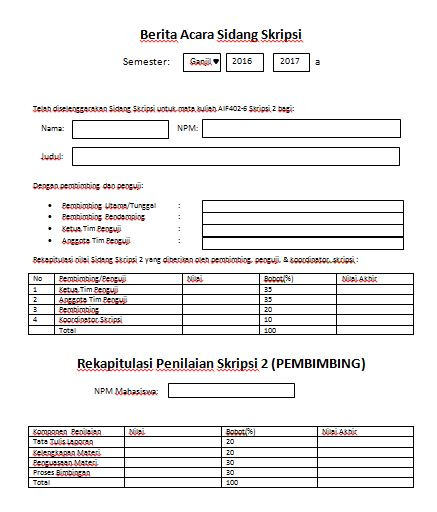
\includegraphics[scale=0.4]{Gambar/tampilan1.png}
		\caption{Perkiraan Tampilan \cite{presentasi}}
		\label{fig:tampilan1}
	\end{figure}
	